\documentclass[a4paper,11pt,twoside]{article}
\usepackage[english]{babel}
\usepackage[utf8]{inputenc}
\usepackage{fancyhdr}
\usepackage[margin=1.2in]{geometry}
\usepackage[T1]{fontenc}
\usepackage{ae,aecompl}
\usepackage[parfill]{parskip} 
\usepackage{subcaption} 
\usepackage{graphicx}
\usepackage{lipsum}
\usepackage{bm}
\usepackage{amsmath,amsfonts,mathtools}
\pagestyle{fancy}
\usepackage[dvipsnames]{xcolor}


\fancyhf{}
\rhead{\textsl{OVERLEAF}}
\lhead{\textsl{GUIDES AND TUTORIALS}}
\renewcommand{\footrulewidth}{0.4pt}% default is 0pt
\fancyfoot[C]{\thepage}
\setcounter{tocdepth}{4}
 
\begin{document}

\tableofcontents
\newpage

\section{Background}
\vspace{6mm}

\subsection{Introduction}

The National Basketball Association (NBA) is a professional basketball league in North America consisting of 30 teams (also called franchises) where each team has of a squad of players called a roster. The teams are evenly split into two `conferences' - the Western Conference and the Eastern Conference. Each team plays 82 games throughout the regular season where they are ranked based off of their win-loss (W-L) record. The top 8 from each conference will then compete in the `playoffs' in an attempt to win the NBA championship. Each franchise is seeded based off of their win-loss record during the regular season and placed in a tournament bracket. Teams with a better win-loss record at the end of the regular season get a higher seeding and are more likely to encounter teams with a lower seeding in the playoffs. In each playoff  round, teams play a best-of-seven game series where the first team to win four games moves into the next round of the playoffs whereas the other team is eliminated. The championship series occurs when the final two teams left in the playoffs play one another in a seven game series. The team which wins this series are the champions of the NBA season.


\subsection{Project Aim and Motivation}

Player statistics are heavily recorded in the NBA as they are a useful indicator of player performance. After every game individual statistics are recorded for every player allowing franchises and basketball enthusiasts to gain an insight about a players contributions throughout the season. Team and individual stats after every game are summarised by a `box score', an example of which is shown in Table 1. Player perfromances are often evaluated using these stat lines and consequently the individual success of a player's season can be defined by inferring from their statistics. In the NBA there are a multitude of statistics and metrics that are recorded; a few examples of the most popular metrics recorded are: \textbf{points scored}, \textbf{assists made} and the \textbf{total number of rebounds}. Furthermore it is also possible to see a trend of a players career by observing the information provided by stat lines from their previous games. For example, it can be speculated that a player is improving if their points, assists and total rebounds per game are increasing. As the success of a team is heavily dependent on individual performances from their players, there is a large motivation for franchises to find players who will improve their team. % !! TALK ABOUT + DIAGRAM OF A BOX SCORE!!
\vspace{5mm}
\begin{table} [h!]
\captionsetup{justification=centering}
\begin{center}
\scalebox{0.55}{
\begin{tabular}{ |c|c|c|c|c|c|c|c|c|c|c|c|c|c|c|c|c|c|c|c|c|} 
 \hline
 Player & MP & FG & FGA & FG\% & 3P & 3PA & 3P\% & FT & FTA & FT\% & ORB & DRB & TRB & AST & STL &BLK & TOV & PF & PTS & +/-\\ 
 \hline
 Jerami Grant & 40:24 & 3 & 14 & .214 & 0 & 3 & .000 & 3 & 4 & .750 & 6 & 8 & 14 & 2 & 0 & 1 & 2 & 1 & 9 & -5\\ 
 \hline
 Paul George & 34:50 & 6 & 14 & .429 & 3 & 10 & .300 & 4 & 7 & .571 & 0 & 5 & 5 & 6 & 1 & 0 & 3 & 6 & 19 & -4\\ 
 \hline
 Russel Westbrook & 43:55 & 16 & 29 & .552 & 5 & 10 & .500 & 5 & 8 & .625 & 2 & 9 & 11 & 6 & 1 & 0 & 9 & 3 & 42 & -7\\
 \hline
 Terrance Ferguson & 33:16 & 3 & 10 & .300 & 2 & 8 & .250 & 0 & 0 & - & 0 & 1  & 1 & 0 & 1 & 0 & 0 & 3 & 8 & -14\\
 \hline
 Steven Adams & 39:58 & 2 & 7 & .286 & 0 & 0 & - & 0 & 0 & - & 7 & 0 & 7 & 2 & 1 & 0 & 2 & 3 & 4 & -4\\
 \hline
\end{tabular}
}
\end{center}
\caption{An Example of an NBA Box Score showing the stats of the Oklahoma City Thunder players who started the game}
\end{table}
%PARA BELOW - DISPLAY WHAT MODELS YOU ARE PLANNING MORE CLEARLY!!!!
This project aims to build on previous studies that explore machine learning models for predicting outcomes in the NBA. Moreover, the focus of this project will be experimenting with different statistical and machine learning algorithms starting with a simple average model and moving to more complex models such as non-linear multi-feature regression in order to accurately forecast the points scored by players over the course of the 2018-19 season. More specifically this project will aim to answer the following questions:

\begin{center}
\textbf{Can machine learning models accurately forecast the points scored for players for every game during the 2018-19 NBA regular season using trends from previous seasons?}

and 

\textbf{Can machine learning models accurately forecasting the average points per game of players for the 2018-19 regular season and thus the general trend of a players career?}
\end{center}
\vspace{7mm}

The contributions of this paper can be summarised as follows:
\begin{itemize}
    \item Selecting the best features for the predictive variable - points scored per game
    \item Outlining, analysing and comparing the different machine learning algorithms used.
    \item Change bullet points
\end{itemize}
%More emphasis on the TIME SERIES ELEMENT!
Essentially, the project aims to solve a \textbf{time series problem} where outcomes in the future are predicted using information given in the present. \textbf{Is it possible to accurately predict the points scored in future games based off the trend of past games played?}

The NBA is a multi-billion dollar industry that is growing in popularity at a fast rate with viewership numbers reaching a record level in the 2017-18 season. The average franchise value is \$1.9 billion, 13\% more compared to the year prior. As a result there is a lot of incentive for franchises to perform well because this would further increase their revenue.

Franchises spend approximately half of their revenue on player salary, and in many ways risk their monetary success on the future of their players when signing them for multi-million dollar long-term contracts. Such monetary risks include team success over multiple seasons, salary cap restrictions, overall franchise value and team marketability. Subsequently the necessity for franchises to accurately forecast future player performance has increased greatly over the recent years in order to acquire players that are most likely to aid their teams success.

The main motivation for this investigation is to help NBA franchises make more informed and well judged decisions when attempting to acquire players. Coaches, scouts and agents can use the models explored  to forecast a particular player's future performances and monitor their development before deciding whether or not to acquire the player. 

Another motivation for exploring this project is the drastic increase in the sports analytics industry and its role in the sports betting market. The sports analytics market is expected to reach \$2.09 billion by 2022, with many more basketball enthusiasts exploring different methods to predict outcomes in basketball games. For example Google Cloud, NCAA and Kaggle hosted the annual `March Madness' competition where basketball fans attempt to forecast outcomes of a college basketball tournament in an attempt to win up to \$10,000.

 Furthermore the sports betting market is so large solely because it is challenging to predict the outcomes of sporting events. As a result, another motivation for exploring this project is to discover a more accurate method of predicting player outcomes to better inform sports betting enthusiasts. 



\subsection{Existing Literature}
 
\subsubsection{ARIMA model Time Series Player Data}

%NEED TO PROOF-READ + MAKE SURE IT MAKES SENSE - potensh add mathematical formulae
This paper explores game-by-game data of one player, Derrick Rose, in order to forecast the number of points scored in upcoming games. More specifically this paper attempts to find the best $ARIMA$ model that best fits Derrick Rose's previous statistics in order to accurately predict the points scored in Rose's future games. - DeLay et al 2016.

The paper uses data from the 2014-15 regular season and as a result the $ARIMA$ models used  were trained using only 51 games of the season (Rose only played 51 games of the regular season, the other 31 were missed due to injury).

$ARIMA(p,d,q)$ stands for Autoregressive Integrated Moving Average and is commonly used in time series analysis where the data displays non-stationary properties, that is the mean and variance changes over time. This model is a generalisation of the $ARMA(p,q)$ model, which combines the autoregressive model with the moving average model. The autoregressive ($AR(p)$) part of the model learns from the previous $p$ games played and uses them as inputs for a regression model to predict the points scored in future games. The moving average ($MA(q)$) model essentially takes the average of the previous $q$ data points. The `integrated' part of the $ARIMA(p,d,q)$ model consists of finding the differences between $d$ data points in order to remove the non-stationary element.

The motivation behind using the $ARIMA$ model is that DeLay assumed there would not be a seasonal trend over the course of the year and as a result the mean and variance of points scored over the course of the season would not change. Another assumption made was that the forecasted points scored by Rose in future games would be similar compared to his previous games implying that there would be no drastic improvement or deterioration in points scored by Rose in the near future.

The results produced in this paper suggest that an an integrated moving average of order 1 ($IMA(1,1)$) best fit Derrick Rose's training data, however the forecasted data was slightly inconclusive. The predicted data points for future games converged to the average of the initial 51 data points. This was potentially due to the fact that the training data set was too small. DeLay believed that over time and given more data the model would predict more fluctuating data points before averaging out at at slower pace. 

%DOESNT MAKE MUCH SENSE RN, NEEDS A PROOF READ BADLY!!

\subsubsection{Weibull-Gamma Statistical Model}

Hwang et al (2012) attempted to forecast the trend of a small subset (7) of player's careers using a different statistical method, namely the Weibull-Gamma model. More specifically, Hwang attempted to forecast the average points per game (PPG) scored by players over the upcoming seasons. The subset of players were all free agents, meaning they were currently not under contract with any particular team in the NBA. This paper aimed to aid NBA franchises such that they could obtain a degree a foresight when deciding whether sign these free agents.


Before Hwang decided to use average PPG over a season as a method for evaluating player performance an array of different features were experimented with to find an accurate metric for player performance. Hwang's reasoning for using the average PPG over the course of a season was because it is a very commonly used statistic. Training data consisted of seven different players, the target variable was the average PPG for a season and the dependent variable was the season number. 

The statistical model used was a mixture of the Weibull-Hazard and the Gamma function. The motivation behind using this model is that the assumption of performance over time is included. In other words, Hwang assumes that player performance will begin to decline as the players partake in more NBA seasons and therefore he is expecting the average points scored per game to decline as more seasons occur.

The results achieved by Hwang after one season of predicting the average PPG for the season upcoming (2010-11) season were fairly encouraging. The difference in points never exceeded more than 2, proving to be a fairly accurate model.

A key difference between Hwang's thesis and the objective in this thesis is that Hwang does not attempt to predict the points scored for individual games throughout a season, only the average points scored per game over the entire season, for multiple seasons in the future. Therefore it can be deduced that this study was focused more on forecasting the general trend of player careers, attempting to decipher the effect of age on a players career rather than attempting to predict the points per game of a player against a particular team

\subsection{The Dataset}

%GO THROUGH THE  PROCESS OF ML: DATA COLLECTION AND PREPROCESSING ->TRAINING -> TESTING -> DISCUSSION AND ANALYSIS

This investigation will focus on a specific subset of players, specifically players from the 2014 Draft Class. The dataset consists of 27 players and their box score statistics from every game over the previous three seasons. The players and the references to the statistics are shown below. The incentive for choosing these players was:
\begin{itemize}
    \item These players are of similar ages and they have had the same number of years of experience in the NBA.
    \item They are still relatively young, so the possibility of a decline in performance due to aging is low.
    \item Although these players are still relatively young, they have played 3 seasons in the league and therefore they should be well adjusted to the difficulty of the NBA.
\end{itemize}
Therefore the assumption made when using this dataset is that it is unlikely that the performance of these players will drastically improve or decline over the course of the 2018/19 season and therefore the points per game for these players may be more predictable.

The data was collected by scraping the box scores off of the website BasketBall Reference. Some box score statistics can be seen as good indicators for predicting the points per game in future games and as a result can be considered as important features. The box score statistics are explained in Table 3.

\vspace{5mm}
\begin{table} [h!]
\begin{center}
\begin{tabular}{ ccccc } 
 \hline
Andrew Wiggins & Jabari Parker & Joel Embiid & Aaron  Gordon& Dante Exum \\ 
 \hline
Marcus Smart & Julius Randle & Nik Stauskus & Noah Vonleh & Elfrid Payton \\ 
 \hline
 Doug McDermott & Zach LaVine & T.J Warren & Jusuf Nurkic & Gary Harris\\
 \hline
 Bruno Caboclo & Rodney Hood & Shabazz Napier & Clint Capela & Kyle Anderson\\
 \hline 
 Joe Harris & Spencer Dinwiddie & Jerami Grant & Glenn Robinson & Nikola Jokic\\
 \hline
  Dwight Powell & Jordan Clarkson\\
\hline
\end{tabular}
\caption{Table consisting of all the players in the dataset}
\end{center}
\end{table}

 \subsubsection{Overview of the Features}
The box scores from every game over the past 3 seasons  were scraped from `Basketball Reference'. Some of the stats recorded could potentially be used a features for forecasting points per game for future games. The features (and the target variable) provided are summarised in the following table. 

\vspace{5mm}
\begin{table} [h!]
\begin{center}
\begin{tabular}{ |c|c| } 
 \hline
MP & Minutes Played  \\ 
 \hline
FG & Field Goals scored \\ 
 \hline
FG\% & Field Goal percentage\\ 
 \hline
3P & Number of 3 point field goals\\
 \hline
 3P\% & 3 point field goal percentage\\
\hline
FT & Number of free throws made\\
\hline
FTA & Number of free throws attempted\\
\hline
FT\% & Free throw percentage\\
\hline
ORB & Number of offensive rebounds\\
\hline
DRB & Number of defensive rebounds\\
\hline
TRB & Total number of rebounds\\
\hline
AST & Number of assists made\\
\hline
STL & Number of steals made\\
\hline
BLK & Number of blocks made\\
\hline
TOV & Number of turnovers conceded\\
\hline
PF & Number of personal fouls conceded\\
\hline
PTS & Number of points scored\\
\hline
GmSc & A score which determines how important a player was in a win\\
\hline
+/- & Net number of points scored when on the court\\
\hline
\end{tabular}
\end{center}
\caption{Table explaining the box score stats}
\end{table}
\vspace{5mm}


There are other factors which could determine the number of points scored by a player in a game which are not captured using just box score statistics. One of these factors is `player form'. This can often be hard to quantify, as there is not a statistic in basketball which quantifies how well a player is performing.  However, a potential way to include form would be use a rolling-window of points scored from previous games, and use this as a feature for predicting the points scored for the upcoming game.  Additionally, another main factor not included in box scores is opponent difficulty. The motivation for including opponent difficulty is that teams vary in defensive capabilities which could impact how many points a player scores in a game.


\subsection{Feature Selection Methods}
In order to improve the performance of the models when predicting the target variable, the most relevant features need to be selected. Feature selection is the approach of selecting the most relevant features for predicting the target variable. It is used because it removes the features which are irrelevant when predicting the target variable and it aids in avoiding the curse of dimensionality. Additionally feature selection enhances generalisation by reducing overfitting. There are many features present in this investigation (examples can be seen in Table 3), however there are some features which may not be pertinent to forecasting the desired target variable in the investigation - points scored. As a result, different feature selection algorithms were explored, namely the 'SelectKBest' algorithm and the Extra-Trees Classifier.


\subsubsection{SelectKBest Algorithm}
The `SelectKBest' algorithm selects a subset of features of size $k$ which have the strongest relationship with the target variable. A wide range of statistical tests can be used to select these features. The statistical test produces a score for each feature, and the top $k$ features which have the highest score the features which have the strongest relationship with the target. For example, a common statistical test used for this algorithm is the chi-squared statistical test.  

 \subsubsection{Feature Importance Using the Extra-Trees Classifier}
 The Extra-Trees Classifier is an algorithm which builds multiple decision trees at random using some of the observations from the training data and the some of the features present in the dataset. This classifier can be used to measure the relative importance of each feature on the predicted variable. The use that the Extra-Trees Classifier provides is that it can produce a `score' for every feature in the dataset, where the higher the score implies the more the correlated that feature is with the predicted variable.


% MAYBE PUT ML ALGOS AFTER INTRODUCING THE DATA SET + FEATURES STUFF
\subsection{Technical Background}
%+ the theory of fitting models to dat aand avoiding overfitting and such!
The following section outlines the theory of the machine learning models used in this project. In addition, the motivation and assumptions made when using these models will also be highlighted:


\subsubsection{Simple Moving Average}
The moving average model is commonly used in time series data. The simple average model essentially uses the previous $n$ data points to forecast future data points by taking the unweighted mean of these $n$ points:
\begin{equation}
\bar{p}_{SMA} = \frac{p_{M} + p_{M-1} + ... + p_{M-(N-1)}} {n} 
= \frac{1}{n} \sum_{i=0}^{n-1}p_{M-i}
\end{equation}

\textcolor{red}{In regards to forecasting points scored by players, the Simple Moving Average assumes that the points scored in the previous $n$ games will be sufficient information when forecasting the points scored in the 2018/19 NBA Season. The Simple Average Model also assumes that a player will score the exact same number of points for every game of the upcoming season, which can be interpreted as a naive assumption.}


\subsubsection{Simple Linear Regression}
Ordinary Least Squares (OLS) or Linear Regression is a linear approach to modelling the relationship between an explanatory variable and the target variable.  Given explanatory variable \(x\) and target variable \(y\), the linear relationship is defined as follows:
\begin{equation}
y(x,w) = w_{0} + w_{1}x
\end{equation}
\textbf{w} (the weight vector) encodes the relationship between the two variables. Simple linear regression attempts to best fit a line to a set of data points by finding values for \textbf{w} which minimises the sum of the squares of the vertical offsets of the points from the line. Essentially the aim is to minimise the following function:
\begin{equation}
L(x) = \sum_{i=0}^{n}(y_{i}-\textbf{w}^Tx_{i})^2
\end{equation}
Where $\textbf{w}^Tx_{i}$ is a point on the line  and \(y_i\) is the data point that is vertical offset from  $\textbf{w}^Tx_{i}$. In order to minimise this function the partial derivative of $L$ is taken and the following derivative is equated to 0. As a result, the following equations encode the values of \(w_{0}\) and \(w_{1}\) which best fit the data points:
\begin{equation}
w_{1} =\frac{\sum{}^{} (x_{i} - \bar{x})(y_{i} - \bar{y})}{\sum{}^{}(x_{i} - \bar{x})^2}
\end{equation}
\begin{equation}
w_{0} = \bar{y} - w_{1}\bar{x}
\end{equation}
where $\bar{y}$ and $\bar{x}$  are the means of the $y$ values and $x$ values.

\textcolor{red}{Concerning this investigation, the target variable will be points scored per game and the explanatory variable will be the game number. Furthermore, Simple Linear Regression will produce a linear trend between the number of games played in the NBA and the points scored per game. As a result, when attempting to forecast the points scored games in the upcoming 2018/19 season, the model will work under the assumption that the points scored in every following game will follow a linear trajectory resembling the trajectory of the fitted line produced from training data (previous seasons). In other words, the points scored in every game will either continue to increase, decrease or the stay the same without any fluctuations throughout the season.}


\begin{figure} [h!]
\captionsetup{justification=centering}
\makebox[\linewidth][c]{%
\begin{subfigure}[b]{.6\textwidth}
\centering
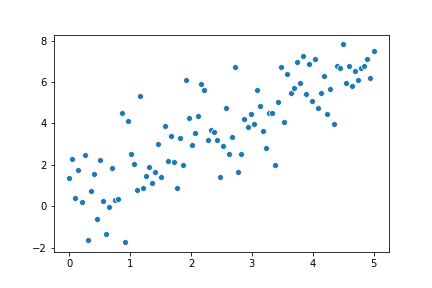
\includegraphics[width=0.95\textwidth]{scatterplt_ex.png}
\caption{Data Points Plotted}
\end{subfigure}%
\begin{subfigure}[b]{.6\textwidth}
\centering
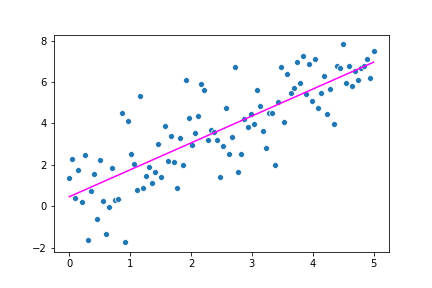
\includegraphics[width=0.95\textwidth]{linregscatterplt.png}
\caption{Linear Relationship calculated}
\end{subfigure}%
}\\
\caption{An example of Simple Linear Regression. The magenta line in Figure 1b) visualises the linear relationship between two variables. It can be seen that the two variables have a positive correlation}
\end{figure}

\subsubsection{Bayesian Linear Regression}
% improve description of theory for Bayesian LS
Bayesian Linear Regression also formulates a linear relationship between the explanatory and target variables, however unlike OLS the relationship is based off a probability distribution rather than point estimates. In other words, the target value is not estimated to be a single value but it is drawn from a specific probability distribution. For this investigation, the weights will be sampled from a Gaussian distribution when computing the target values. The reasoning behind this stems from the Central Limit Theorem. This model uses Bayes Theorem to produce probability distribution for the target values - called the posterior. A probability encoding an existing or prior belief of the weights (also called parameters) is multiplied by the likelihood of the data points. It is then divided by a normalisation constant. The prior belief will be a Gaussian distribution, and due to conjugacy, the posterior will also follow a Gaussian distribution. 
\begin{equation}
 y \sim N(\textbf{w}^T\textbf{X}, \sigma^2\textbf{I})
\end{equation}
\begin{equation}
P(\textbf{w}|y,\textbf{X}) = \frac{P(y|\textbf{X},\textbf{w})P(\textbf{w})}{P(y|\textbf{X})}
\end{equation}
One of the benefits of using Bayesian linear regression is that a prior belief about the model parameters can be specified, rather than assuming that all the information regarding the parameters is included within the data set. Another benefit of Bayesian linear regression is that uncertainty is included in our model due to the fact that the posterior is a probability distribution. If the dataset is small the posterior distribution of the parameters will be more spread out. Therefore it can be implied that the model is more uncertain in its belief of parameter values. As more data points are observed the posterior probability is `updated' and the model becomes more certain concerning its parameter values. If infinite data points were to be observed, the prior probability would essentially be washed out, and the best fitting line would converge to the OLS best fitting line.

\textcolor{red}{The main motivation for including this model in this investigation is that a prior belief about the trajectory a particular player's upcoming season.}

\subsubsection{Kernel Ridge Regression}
%TEMPORARY - GET RID OF THIS LATER
Kernelised Ridge Regression is a nonlinear approach for modelling the relationship between an explanatory variable and a target variable. It combines Ridge Regression with the `kernel trick'.

Ridge Regression is similar to Least Squares Regression where a curve is best fitted to a set of data points through minimising a loss function specified by Equation (2). However, the major risk when attempting to fit a curve to data is overfitting. One simple method for avoiding overfitting is to include penalty term to \textbf{w} in the loss function. Subsequently the loss function becomes, 
\begin{equation}
L = \sum_{i=0}^{n}y_{i} - \textbf{w}^Tx_{i} + \lambda||\textbf{w}||^2
\end{equation}
$\lambda$ is the regularisation parameter. If $\lambda$ were to be zero, then the loss function function would be the same as the loss function for least squares.

\begin{figure} [h!]
\makebox[\linewidth][c]{%
\begin{subfigure}[b]{.6\textwidth}
\centering
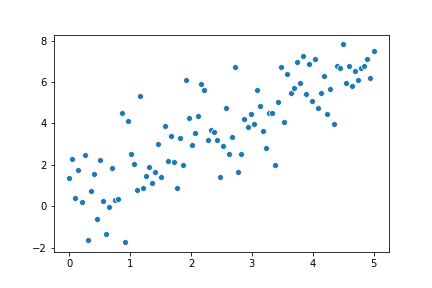
\includegraphics[width=0.95\textwidth]{scatterplt_ex.png}
\caption{Data Points Plotted}
\end{subfigure}%
\begin{subfigure}[b]{.6\textwidth}
\centering
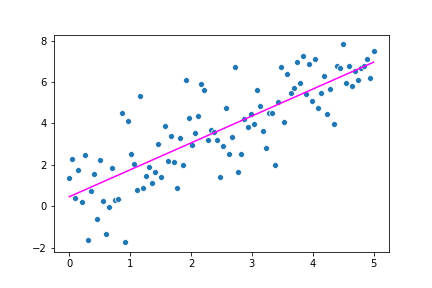
\includegraphics[width=0.95\textwidth]{linregscatterplt.png}
\caption{Linear Relationship calculated}
\end{subfigure}%
}\\
\caption{Different values of $\lambda$}
\end{figure}


In order to achieve a nonlinear curve a kernel function, $k(x,x')$ is applied to all input values. Kernel functions describe the inner product of two input values that are mapped to a different feature space $\mathcal{X} \rightarrow \mathcal{F}$: $k(x_{1},x_{2}) = \phi(x_{1})^T\phi(x_{2})$. The basis function $\phi(.)$ is unknown however it is not required as long as the mapped feature space is an inner product space; this is known as the kernel trick The idea behind using kernels is that when the inputs are mapped to a different feature space, they can be classified linearly as seen in Figure 3. Examples of kernel functions include the Radial Basis Function, the Polynomial Kernel and the  Fisher Kernel.

      \begin{figure}[!htb]
      \captionsetup{justification=centering}
        \center{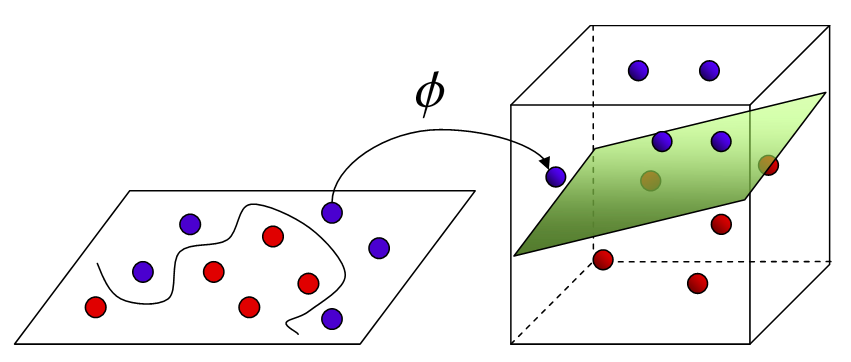
\includegraphics[width=0.6\textwidth]
        {kerneltrick.png}}
        \caption{\label{fig:my-label}By applying a basis function, the data points are mapped from a 1-dimensional feature space to a 2-dimensional feature space, where it can be linearly separated}
      \end{figure}

\textcolor{red}{The main motivation behind using Kernel Ridge Regression in this investigation is that the trajectory of a players performance over games played may not be linear. For example, a number of points scored by a player may have improved exponentially over last 20 games, and therefore applying a non-linear curve to this data may better fit the trajectory of his career. It can be inferred that this model will place more emphasis on recent form when attempting to forecast future results.}

\begin{figure} [h!]
\captionsetup{justification=centering}
\makebox[\linewidth][c]{%
\begin{subfigure}[b]{.45\textwidth}
\centering
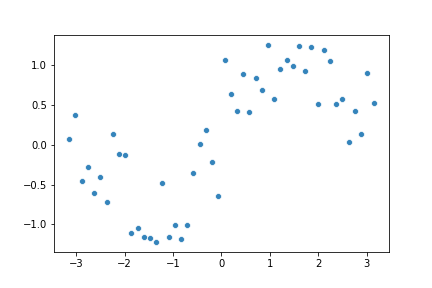
\includegraphics[width=0.95\textwidth]{wavey.png}
\caption{}
\end{subfigure}%
\begin{subfigure}[b]{.45\textwidth}
\centering
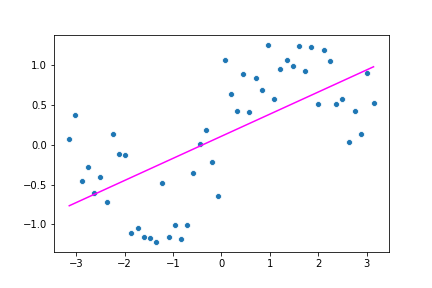
\includegraphics[width=0.95\textwidth]{wavey_lr.png}
\caption{}
\end{subfigure}%
\begin{subfigure}[b]{.45\textwidth}
\centering
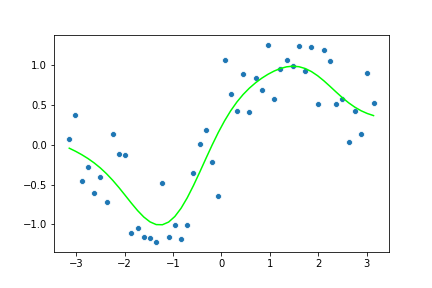
\includegraphics[width=0.95\textwidth]{wavey_kr.png}
\caption{}
\end{subfigure}%

}\\
\caption{The relationship between the two variables are not linear, therefore, attempting to use a linear regression would result in a poor fit of the data observed in b). Kernel ridge regression produces a non-linear curve which better fits the relationship between the two variables, seen in c)}
\end{figure}

\subsubsection{Multiple Linear Regression and Multivariable Kernel Ridge Regression}

Multiple Linear Regression models a relationship between more than one explanatory variable and a target variable by fitting a linear equation to the observed data:
\begin{equation}
y_{i} = w_{0} + w_{1}x_{i} + w_{2}x_{i} +  ... + w_{d}x_{i}
\end{equation}
A feature matrix consisting of the explanatory variables $\textbf{X}$ and a column vectors consisting of the target variable $y$ and weights $\textbf{w}$ can be represented as:
\[
\begin{bmatrix}
	y_{1}\\
	y_{2}\\
	\vdots \\
	y_{d} \\
\end{bmatrix}
= \begin{bmatrix}
    x_{11} & x_{12} & x_{13} & \dots  & x_{1n} \\
    x_{21} & x_{22} & x_{23} & \dots  & x_{2n} \\
    \vdots & \vdots & \vdots & \ddots & \vdots \\
    x_{d1} & x_{d2} & x_{d3} & \dots  & x_{dn}
\end{bmatrix}
\begin{bmatrix}
	w_{1}\\
	w_{2}\\
	\vdots \\
	w_{d} \\
\end{bmatrix}
\]
In order to establish a linear relationship between $y$ and $\textbf{X}$ the weights are calculated using the least squares method akin to simple linear regression. Therefore the following loss function that needs to be minimised is $Xw -y^2$. The formula for finding the weights which minimises the loss function is
\begin{equation}
\textbf{w} = (\textbf{X}^T\textbf{X})^{-1}\textbf{X}^Ty
\end{equation}
\textcolor{red}{Within the context of this investigation, Multiple Linear Regression allows for different features other than just games played over time. For example, if a player is playing against a team who is less defensively adept compared to other teams, the player may score more points in that particular match compared to the other teams, or a player may have recently hit a good patch of form over the past few games, it is therefore logical to assume he will score more points in the next game. Using more features may allow for a more accurate prediction of player points per game. Multiple Linear Regression assumes that each explanatory variable is independent from another.}

Multivariable Kernel Ridge Regression is a simple extension of its single feature counterpart. Additionally, like Multiple linear regression there is or than one explanatory variable describing the target variable. 

 \subsubsection{Training and Test Data}
Machine learning models are initially fit on a training dataset. The training data consists of a set of explanatory variables and the respective target variables. The model essentially learns from this data and fits its parameters to the training data. After the model is trained, its performance is assessed using a test dataset. If the models performance of the training data is is similar to that of the test data.

\subsubsection{Overfitting}
When attempting to fit a machine learning model to data, it is important that overfitting is avoided. Overfitting occurs when the machine learning algorithm attempts to learn the noise within the dataset as well as attempting to learn the signal presented in the dataset. Noise in a dataset refers to the randomness within a dataset and signal refers to the underlying pattern in the dataset that wish to learn.One approach of detecting overfitting when learning is to plot the validation error of the training data and the test data. If the validation error begins to increase for the test data while decreasing for the training data then the model has most likely over fitted the training data. 

      \begin{figure}[!htb]
      \captionsetup{justification=centering}
        \center{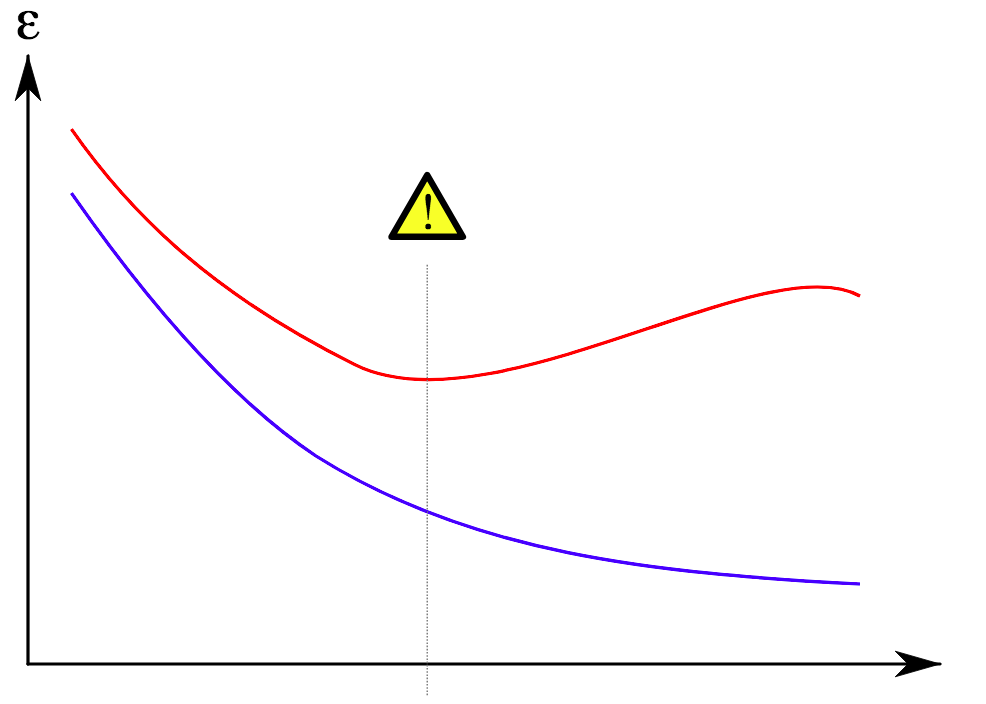
\includegraphics[width=0.6\textwidth]
        {overfitpng.png}}
        \caption{\label{fig:my-label} A visualisation of overfitting. The red line represents the error of the testing data whereas the blue line represents the error. If there is an attempt to completely minimise the training data's error, then the model will become less flexible when attempting to predict future data points, resulting in an increase in the testing data's error. }
      \end{figure}

\subsubsection{Root Mean Squared Error}
This investigation will use the Root Mean Squared Error (RMSE) quantify the error in each model. RMSE is that standard deviation between the values predicted by a machine learning model and the values observed.
\begin{equation}
RMSE = \sqrt[]{\frac{\sum_{i=0}^{n}(\hat{y}_{i} - y_{i})}{n}}
\end{equation}
In order to check whether a model has over fit or underfit the data, the RMSE from the training data and the RMSE of the test data will be compared. If the RMSE is drastically higher for the test data compared to the training data then the model has over fit the data. If the RMSE for both sets are similar then the model has fit the data well. 

Additionally, the RMSE can be used to compare the efficacy between models. Models with a lower RMSE compared to others imply that they're better at forecasting the trajectory of player points per game compared to models which score a higher RMSE.



\newpage

\section{Methodology and Implementation}

After data was collected for each player, the data was placed in an array and preprocessed. Certain games were removed in order to avoid the data from being skewed. For example, if a player had played only a small number of minutes of a game due to unforeseen circumstances such as obtaining an injury, it would be removed from the dataset. Player form was also added to the array. It was decided that the points scored per game over a certain number of games were added. Furthermore opponent difficulty was also added to the array using the defensive rating metric provided by the NBA.

Scatter plots depicting the points scored over games played were then made in order to visualise the relationship between these two variables before they were trained by the machine learning models.The figures also show the Least Squares Regression plot of two of the players in the dataset. Figures 6a) and 6b) are the scatter plots for two players, Joel Embiid and Nikola Jokic. As visualised in these figures the variance of points scored over a game-by-game basis is very large, thus potentially making the task of predicting the exact number of points scored by players in a particular game a very challenging task. However a general trend can be deduced from these graphs. There is a weakly positive correlation between number of games played and points, therefore it can hypothesised that for the upcoming season, this trend will continue. Some models in this investigation consist of one explanatory variable and a target variable, these include the Simple Moving Average model, Simple Linear Regression, Bayesian Linear Regression and Kernel Ridge Regression.


\begin{figure} [h!]
      \captionsetup{justification=centering}
\makebox[\linewidth][c]{%
\begin{subfigure}[b]{.7\textwidth}
\centering
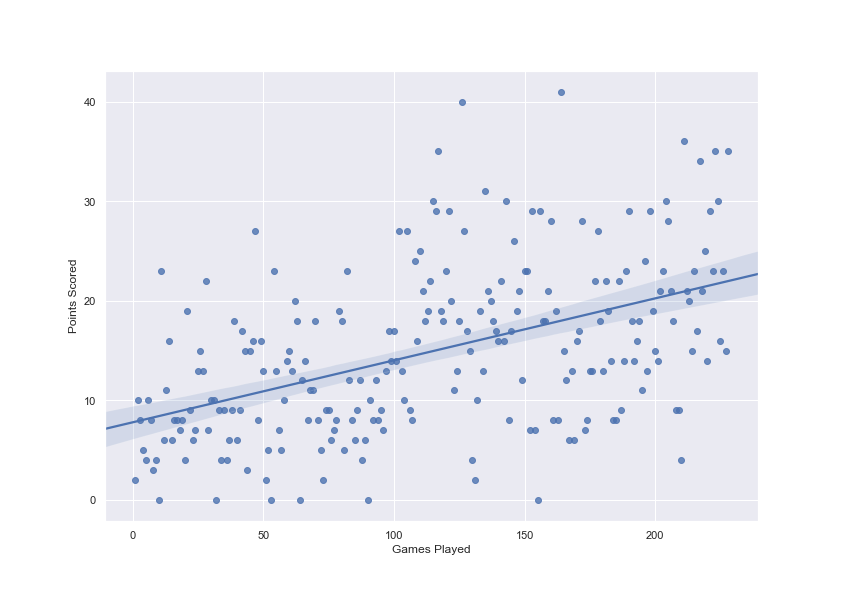
\includegraphics[width=1.05\textwidth]{../players/player24.png}
\caption{Graph visualising Nikola Jokic's points scored}
\end{subfigure}%
\begin{subfigure}[b]{.7\textwidth}
\centering
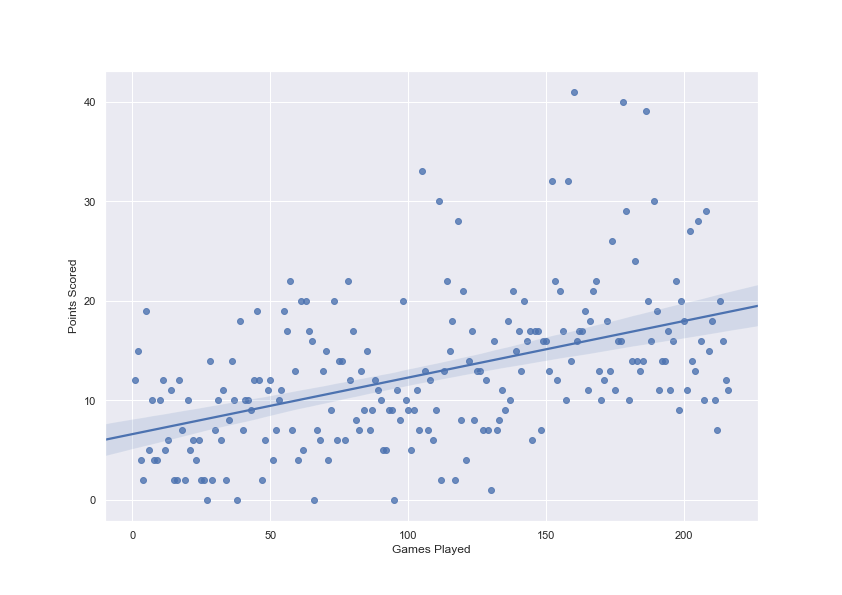
\includegraphics[width=1.05\textwidth]{../players/player3.png}
\caption{Graph visualising Aaron Gordon's points scored}
\end{subfigure}%
}\\
\caption{The two Figures above visualise the relationship between the points scored of two players in the dataset over the course of their career's so far. The blue line shows the regression represents the linear relationship between the two variables and the shaded blue region represents one standard deviation.}
\end{figure}



\subsection{Feature Selection}

Feature selection is required for the models which use multiple features. Using more features may allow us to explain the target variable better and produce more accurate results when forecasting points per game.  Pair plots were produced to see if there was a correlation between a feature and the target variable. 

As stated earlier the features used to predict the points scored in future games consist of the box score statistics of the previous game, as well as the current opponent for that particular game. Examples plots of some of the features for Nikola Jokic can be seen below. The results when visualising the correlation between the features and the target variable suggest that there is no correlation between the points scored and the opponent difficulty, explaining that that the number of points scored for a player is independent of opponent. Additionally the same results can be concluded for the plus-minus (+/-) statistic. However, other features such as field goal attempts (FGA), minutes played (MP) and a players GameScore (GmSc) present weakly positive correlation. This would indicate that these features aid in forecasting a players points per game. 


\begin{figure} [h!]
\makebox[\linewidth][c]{%
\begin{subfigure}[b]{.45\textwidth}
\centering
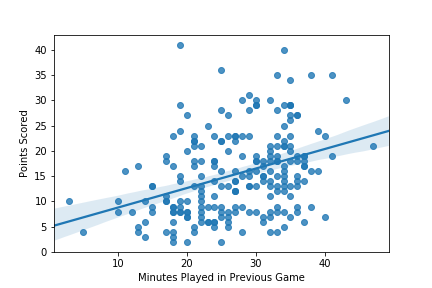
\includegraphics[width=0.95\textwidth]{../mp_pts.png}
\caption{Minutes Played}
\end{subfigure}%
\begin{subfigure}[b]{.45\textwidth}
\centering
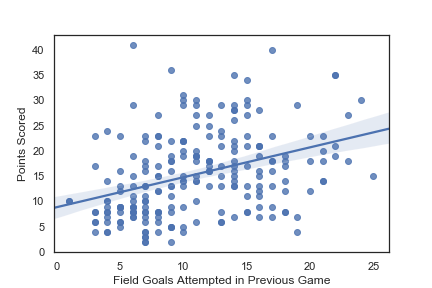
\includegraphics[width=0.95\textwidth]{../fga_pts.png}
\caption{Field Goals Attempted}
\end{subfigure}%
\begin{subfigure}[b]{.45\textwidth}
\centering
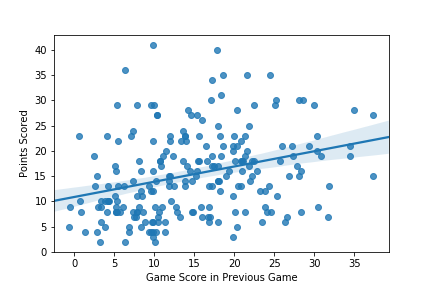
\includegraphics[width=0.95\textwidth]{../gmsc_pts.png}
\caption{GameScore}
\end{subfigure}%
}\\
\caption{The Figures above visualise the relationship between points scored in a game and specific stats from the prior game. This was done to see if there was a positive correlation between these features and the target variable. The Figures shown are taken from one player in the dataset }
\end{figure}


\begin{figure} [h!]
\makebox[\linewidth][c]{%
\begin{subfigure}[b]{.45\textwidth}
\centering
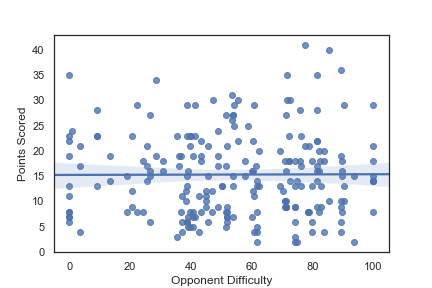
\includegraphics[width=0.95\textwidth]{../opp.png}
\caption{Opponent Difficulty}
\end{subfigure}%
\begin{subfigure}[b]{.45\textwidth}
\centering
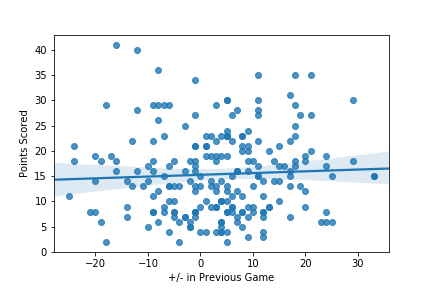
\includegraphics[width=0.95\textwidth]{../pminus_pts.png}
\caption{+/- Score}
\end{subfigure}%
\begin{subfigure}[b]{.45\textwidth}
\centering
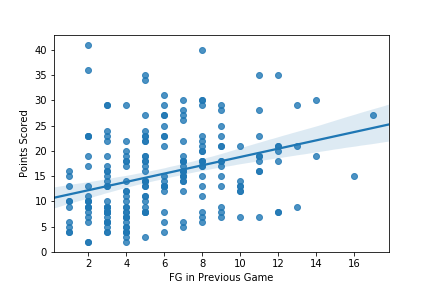
\includegraphics[width=0.95\textwidth]{../fgoals_pts.png}
\caption{Field Goals Scored}
\end{subfigure}%
}\\
\caption{More features plotted to see if they are correlated to  the number of points scored.}
\end{figure}



After visualising the correlation between the features and the target variable, the feature selection methods outlined in the previous chapter were applied to the dataset. After applying these methods, the final subset of features will consist of those which best forecast the points scored.

\subsection{Results using Select K Best}

The datasets of each players statistics were subjected to the Select K Best Algorithm where the $k$ most correlated features with points scored using the chi-squared test was selected. The question that arises when using this algorithm is how many features should we select? This is explored more in the upcoming chapters, however the general logic of combatting this issue was increasing the value of $k$, applying the $k$ number of features to the model and recording the RMSE. If by adding more features, the RMSE for the training and test data increases, then the number of features will be reduced. After applying the Select K Best to all player datasets, the most correlated feature was number of games played, followed by points scored from the previous 3 games. The next two features selected was the Game Score and the Field Goals attempted from the previous game.

\subsection{Results Using the Extra-Tree Classifier}

The results obtained when selecting the most relevant features using the Extra-Trees classifier was extremely similar to the features obtained using the SelectKBest algorithm. For most players, the features which were highly correlated with points scored for certain games were the number of games played, the players GameScore and the previous games played. However, due to the randomised nature of the extra trees classifier, on a few iterations of the algorithm, one of the highly correlated features for certain players consisted of the players plus-minus (+/-) from the previous game and the opponent they were currently playing. Examples of these are shown in the figures below. As a result, these features were also experimented with and applied to the machine learning models in order to see whether they yielded more accurate results.



\begin{figure} [h!]
 \captionsetup{justification=centering}
\makebox[\linewidth][c]{%
\begin{subfigure}[b]{.55\textwidth}
\centering
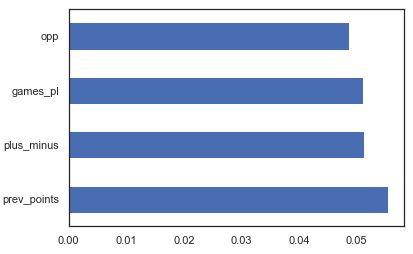
\includegraphics[width=0.85\textwidth]{etc1.png}
\caption{One iteration of Extra-Trees Classifier}
\end{subfigure}%
\begin{subfigure}[b]{.55\textwidth}
\centering
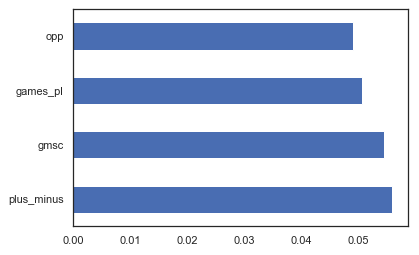
\includegraphics[width=0.85\textwidth]{etc2.png}
\caption{Another iteration of Extra-Trees Classifier}
\end{subfigure}%
}\\
\caption{The bar charts show two different iterations of the extra-tree classifier for one player. When attempting to choose the 4 most correlated features, some features were selected in one iteration and not selected in another. As a result, the models were applied with both sets of features to see which one resulted in the lowest RMSE}
\end{figure}

After the relevent features had been selected, the machine learning models outlined in Chapter 1.6 were then trained and tested. The next chapter entails the results of this investigation: 

\newpage

\section{Results}

After the models learned the training data, they were evaluated using the test dataset - the results are shown below. Table 4 shows the average RMSE of each model when predicting points scored per game for every player in the dataset for the 2018/19 season.

Table 5 depicts the models RMSE for predicting for players season average points per game. In other words, the points predicted for each game of a player is averaged and compared to the observed season average the player scored. This table can be used to see the overall players trajectory for the season, and often determines whether a player had a successful season.
\vspace{5mm}
\begin{table} [h!]
\captionsetup{justification=centering}
\begin{center}
\begin{tabular}{ |c|c|} 
 \hline
 \textbf{Model} & \textbf{Mean RMSE}\\ 
 \hline
 Simple Moving Average &  6.71\\ 
 \hline
 Simple Linear Regression &  6.39\\ 
 \hline
 Bayesian Linear Regression& 6.90\\
 \hline
 Kernel Ridge Regression& 6.27\\
 \hline
 Multiple Linear Regression& 6.60\\
 \hline
 Multivariable Kernel Ridge Regression & 6.27\\
 \hline
\end{tabular}
\end{center}
\caption{Results when attempting to forecast the points scored for every player on a game by game basis}
\end{table}

\begin{table}[h!]
\captionsetup{justification=centering}
\begin{center}
\begin{tabular}{ |c|c|} 
 \hline
     \textbf{Model} & \textbf{Mean RMSE}\\ 
 \hline
 Simple Moving Average  & 3.80\\ 
 \hline
 Simple Linear Regression & 3.13\\ 
 \hline
 Bayesian Linear Regression  & 3.73 \\
 \hline
 Kernel Ridge Regression  & 2.86\\
 \hline
 Multiple Linear Regression& 3.13\\
 \hline
 Multivariable Kernel Ridge Regression  & 2.90\\
 \hline
\end{tabular}
\end{center}
\caption{Results when attempting to forecast season average points per game in the 18/19 season}
\end{table}

\subsection{Simple Moving Average}

The simple moving average, arguably the most naive method used in this investigation, took  the mean of the last 'n' games and assumed that future points scored would be the average produced. Choosing the size of $n$ seemed to be a challenging task. In order to find the n which resulted in the lowest RMSE when predicting the points of every game in the 18/19 season, different values of n were experimented. The size of 'n' which resulted in the lowest RMSE was 20, suggesting that the previous 20 games were the most accurate when using this model to forecast future points scored per game. Example plots forecasting the points scored for the 2018/19 can be seen in Figure 10.

\begin{figure}
\captionsetup{justification=centering}
\makebox[\linewidth][c]{%
\begin{subfigure}[b]{.7\textwidth}
\centering
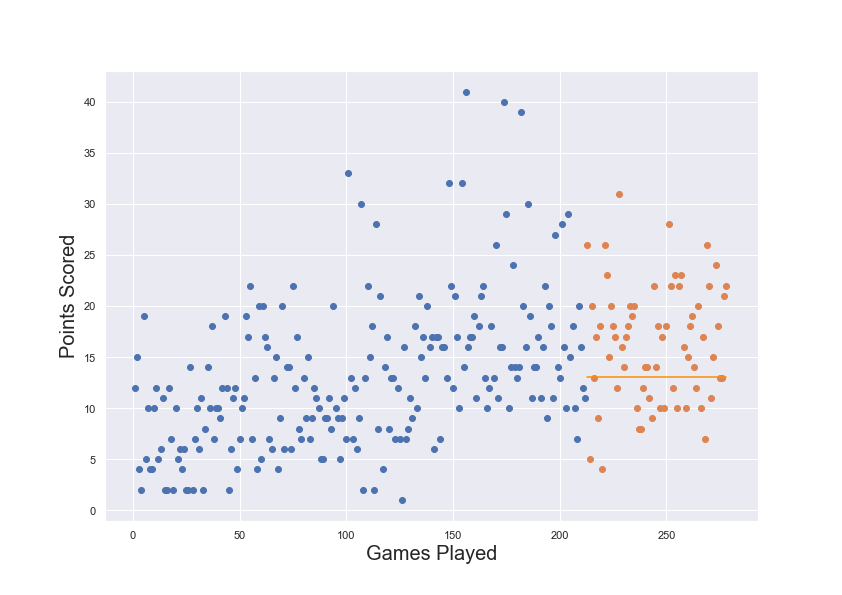
\includegraphics[width=1.05\textwidth]{../players_sma/player3.png}
\caption{SMA results for Aaron Gordon}
\end{subfigure}%
\begin{subfigure}[b]{.7\textwidth}
\centering
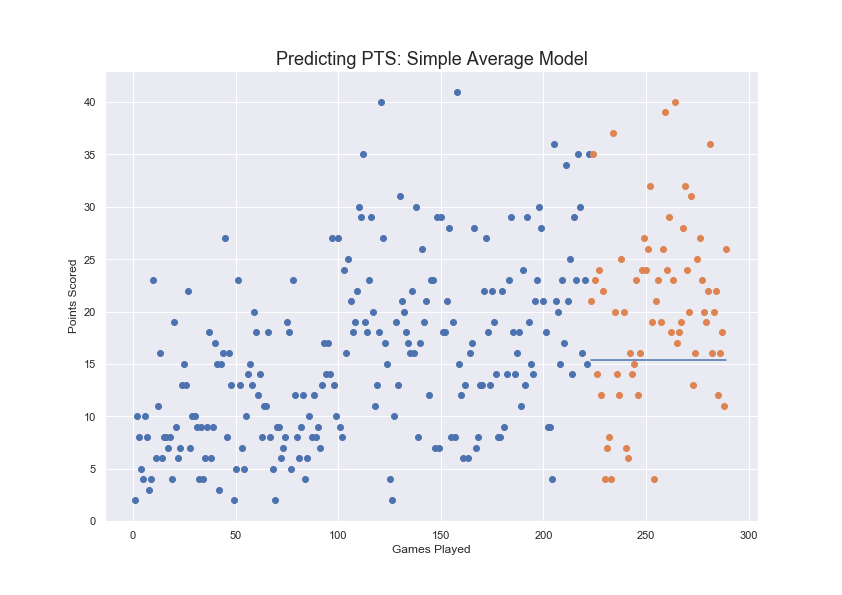
\includegraphics[width=1.05\textwidth]{../players_sma/player24.png}
\caption{SMA results for Nikola Jokic}
\end{subfigure}%
}\\
\caption{These Figures show the results of the SMA model. The blue data points represents the training data points. The orange line depicts the prediction of the SMA model. The orange data points are the points actually scored by the players in the 18/19 season}
\end{figure}

\subsection{Simple and Bayesian Linear Regression}

Simple Linear Regression resulted in a lower RMSE compared to the simple moving average model, implying that this model is a better fit to the data compared the previous model. Example plots of two players are shown in Figure 11. 


\begin{figure} [h!]
\captionsetup{justification=centering}
\makebox[\linewidth][c]{%
\begin{subfigure}[b]{.7\textwidth}
\centering
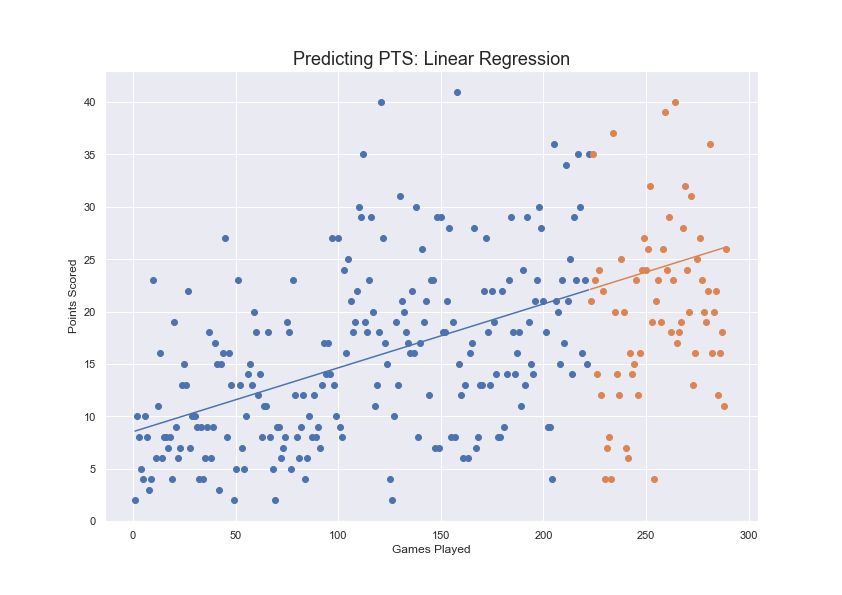
\includegraphics[width=1.05\textwidth]{../players_lr/player24.png}
\caption{Linear Regression - Nikola Jokic}
\end{subfigure}%
\begin{subfigure}[b]{.7\textwidth}
\centering
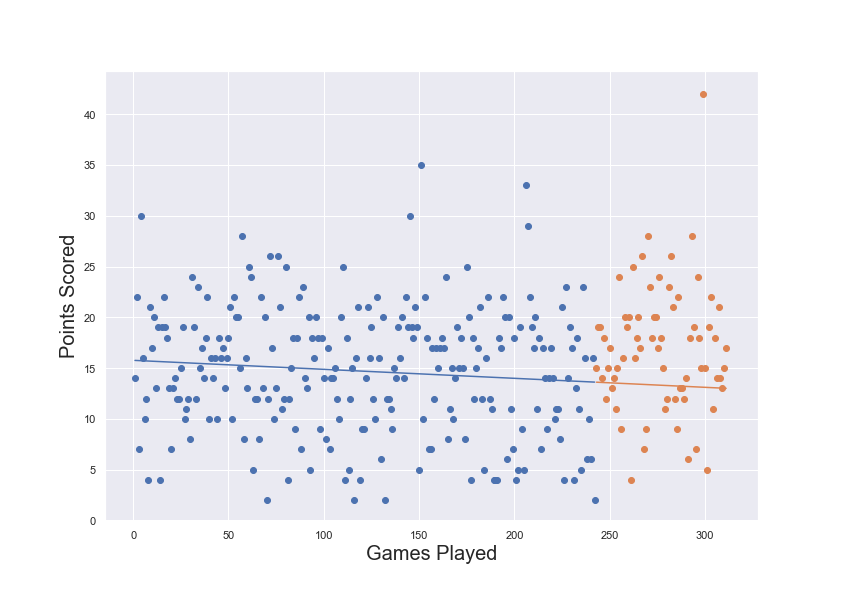
\includegraphics[width=1.05\textwidth]{../players_lr/player26.png}
\caption{Linear Regression Jordan Clarkson}
\end{subfigure}%
}\\
\caption{These Figures show the results of the simple linear regression model. The blue data points represents the training data points. The blue line depicts the best fitting line of the training data and the orange line is the predicted points scored for every game in the 2018/19 season. The orange data points are the points actually scored by the players in the 18/19 season}
\end{figure}

On the other hand, Bayesian Linear Regression produced the highest RMSE out of all the other models in this investigation.

\subsection{Kernel Ridge Regression}

Kernel ridge regression produced a lower RMSE compared to the other investigation, however choosing the correct regularisation parameter was key in finding the best fitting model whilst also avoiding overfitting of the training data. The results produced suggest that a non-linear curve fits the relationship between the games played and points scored better than a linear fit.


\begin{figure} [h!]
\captionsetup{justification=centering}
\makebox[\linewidth][c]{%
\begin{subfigure}[b]{.7\textwidth}
\centering
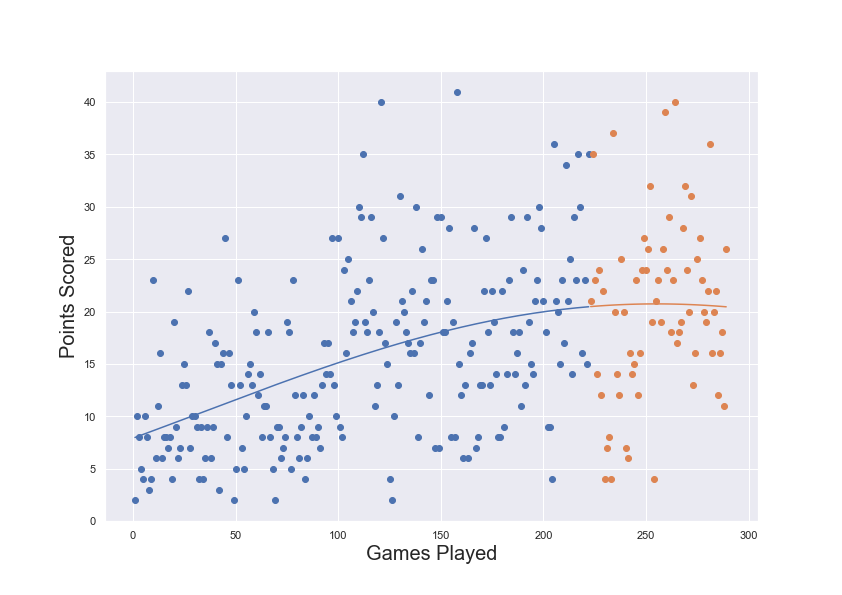
\includegraphics[width=1.05\textwidth]{../players_krr/player24.png}
\caption{Kernel Ridge Regression - Nikola Jokic}
\end{subfigure}%
\begin{subfigure}[b]{.7\textwidth}
\centering
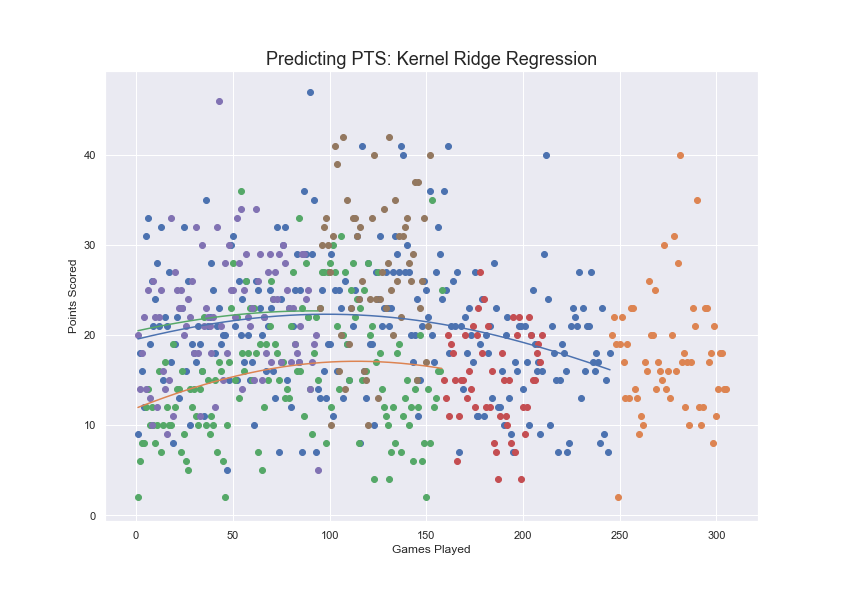
\includegraphics[width=1.05\textwidth]{../players_krr/player2.png}
\caption{Kernel Ridge Regression - Joel Embiid}
\end{subfigure}%
}\\
\caption{The Figures show the training data points and the forecasted plots for Nikola Jokic and Joel Embiid.}
\end{figure}

\subsection{Multivariable Linear Regression and Kernel Ridge Regression}
Multivariable  linear regression produced a larger error value compared to its simple counterpart, however multivariable kernel regression produced extremely similar results to single feature kernel ridge regression. As stated in the previous section, the features selected were points scored from previous games, as well as the number of FGA attempts and the Game Score from the previous games.

When looking at Table 4, we can see that the models varied in accuracy compared to one another. We can see that both simple Kernel Ridge Regression and Multivariable Kernel Ridge Regression were the most accurate for forecasting the points scored on a game by game basis - however, the difference in error values are small.

Single feature Kernel Ridge Regression produced the lowest error when forecasting the average points scored of players in the 2018/19 season regarding points scored.

\newpage
\section{Discussion and Analysis}

\subsection{Game by Game and General Trend Analysis}
Firstly, the average RMSE for each model ranges from 6.27 - 6.90 points per game for the players in the dataset. This implies that predicting the exact number of points scored in a game using these models is a challenging task. The number of points scored on a game by game basis can vary and fluctuate by a large amount, and these models were not able to capture these fluctuations. An example of that occurred this season was when Nikola Jokic scored a season high 40 points in the 42nd game of the season, but the models used in this investigation predicted he would only score between 20 to 23 points per game, which is within the range of points that Jokic had scored in the previous 3 games. 

However, on the other hand, predicting the season average of points scored for the players resulted in a lower RMSE. Thus, it can be argued that the models performed better when attempting to decipher the average of the number of points scored by a player over a season compared to every individual game in a season. Therefore, these models achieved reasonable success when attempting to give foresight in overall future performance. This can be useful for NBA franchises when they are attempting to forecast a particular player?s average points scored for an upcoming season.

The results produced by the regression models for predicting the season average points scored were more accurate for some players compared to other players which suggests that the regression models fit the trajectory of a players career better than other other players. For example, the kernel regression model forecasted that Nikola Jokic would average 20.9 points per game which was close to the 20.1 points per game he achieved. On the other hand, this model predicted Joel Embiid would average 22.3 points per game based off of all of his career games, however he managed to achieve a season average of 27.5 points per game, 5.2 points greater than the prediction and a much larger average compared to his previous seasons. This example shows that these models are not able to anticipate large changes in player form for future seasons.


\subsection{Comparing the Models}
When choosing the model which best fits the data, the results show that single feature kernel ridge regression produced the lowest RMSE when attempting to predict points scored for every game of the 18/19 NBA season as well forecasting the average points scored per game all players included in the dataset.

These results suggest that the trend of player performance over the course of his career is not linear. The plots confirm this assumption and can be seen in Figure 12a) (Nikola Jokic) where this players points scored initially increases at a reasonable rate as the number of games played increases, however the rate of increase of points scored begins to plateau before the upcoming season. Therefore this model predicts that the number of points scored for the 2018/19 season will follow this trend.

A potential reason why the kernelised regression models produces a slightly lower RMSE compared to the linear models is the assumption that games played closer to the 18/19 season hold more importance compared to the games played early on in a players career. Linear regression attempts to find a best fitting linear relationship between the explanatory and target variable using all the data points, however, data points from games which are early in a players career may not be representative for a players career compared to later games.

When comparing the single feature models to the multivariable models, the results display that the single feature methods produce a similar or even a lower RMSE compared to their multivariable counterparts. The results here suggest that the number of games played is sufficient enough to produce the most accurate forecasting of points scored as possible, and that the additional features included do not further improve accuracy of the results.

However, having stated the above, the RMSE for each model are extremely close between one another when predicting game by game results and season average results. All regression models performed similarly to one another, and it  can be argued that no model is significantly more accurate than one another.


\subsection{Limitations}
There were many limitations involved when attempting to predict the target variable. Firstly, capturing player form as a feature proved to be difficult. As explained before, this investigation used points scored from a specific number of previous games. However, this assumption made does not completely capture the tangible form of a player. For example, this assumption would not be able to foresee whether a player has an ?off-game? and doesn?t manage to score as many points as usual. Additionally, players often have a busy schedule and can get fatigued or tired when playing multiple games in a short amount of time and thus can affect the number of points scored in a game. This was not taken into account in this investigation. Also, although none of the players in the dataset did suffer from any long term injuries, if NBA franchises were to use these models to forecast player performance , it would not be able to forecast any injuries that players may get. 

However, one factor that it is believe did in fact limit the results, is that certain players did change teams for the 2018/19 season. The reason this could affect the results is because the players role may change if he changes team. For example, if the player changes team which has better players compared to his former team, he may not play as much per game and as a result the number of points the player scored may decrease. Additionally, changing team also means changing teammates. As a result, teammate chemistry would have changed and this could have directly affected the point scored by the players. An example of this occurring in the dataset was Julius Randle, where he moved from the Los Angeles Lakers to the New Orleans Pelicans. Resultantly, Randle?s average points per game for the season increased dramatically from the previous season (16.1 points per game to 21.4). These models were not able to quantify the effect of a player changing teams and as a result would limit the results for players in this circumstance.

\subsection{Overfitting Problem}
As stated before, avoiding overfitting is key when attempting to forecast future outcomes when using machine learning models. The RMSE of the training data was compared to the test data.


\begin{table}[h!]
\captionsetup{justification=centering}
\begin{center}
\scalebox{0.8}{
\begin{tabular}{ |c|c|c|} 
 \hline
 \textbf{Model} & \textbf{Mean RMSE of Training Data} &\textbf{Mean RMSE of Test Data}\\ 
 \hline
 Simple Moving Average & 5.91 &  6.71\\ 
 \hline
 Simple Linear Regression & 5.69 &  6.39\\ 
 \hline
 Bayesian Linear Regression& 6.01 & 6.90\\
 \hline
 Kernel Ridge Regression& 5.50 & 6.27\\
 \hline
 Multiple Linear Regression& 5.67 & 6.60\\
 \hline
 Multivariable Kernel Ridge Regression & 5.47 & 6.27\\
 \hline
\end{tabular}
}
\end{center}
\caption{Comparing the RMSE of the training data and the testing data for every model}
\end{table}
\vspace{5mm}

\subsubsection{Picking the correct Regularisation parameter}

For the kernelised methods, it was vital that the correct regularisation parameter was selected in order to prevent overfitting. When experimenting with different values, it was concluded that higher values of lambda resulted in an overfitting of the training data and thus resulted in a poor fit for the test data. However, on the other hand, if the regularisation parameter was too low, the models would under fit the training data and as a result the RMSE for the test data would be high. As a result the regularisation parameter was chosen by looping through different values, and choosing the value which resulted in the lowest RMSE for the training and testing data. The graph below show the testing data?s RMSE for single feature kernel regression and multi feature kernel regression with varying values of lambda. 

      \begin{figure}[!htb]
        \centerline{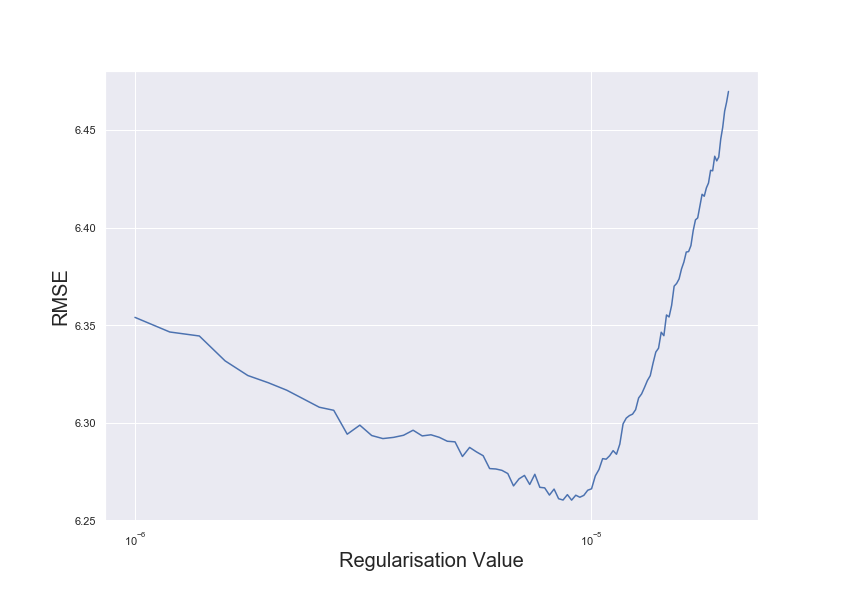
\includegraphics[width=0.7\textwidth]
        {../errvals.png}}
        \caption{\label{fig:my-label} The RMSE of the testing data for Kernel Ridge Regression with different regularisation values}
      \end{figure}


It can be seen in Figure 13 that there is a fall in the RMSE as the regularisation parameter increases, but as the regularisation parameter rises past a certain value, the RMSE begins to increase suggesting that the model has overfit the training data.



\subsection{Choosing Correct window for form}

As stated earlier, when attempting to forecast the points scored from a game, one of the features was player form. In order to capture player form the points scored from a ?window? of games were included. However choosing the number of games to use in this window proved to be a challenging task. The method to combat was to vary the window size and see which window size would result in the lowest average RMSE. In other words, the number of games used to explain player performance were experimented with. The chart below depicts the average RMSE for the multivariable models when different sized windows were used. 

\vspace{5mm}
\begin{table}[h!]
\captionsetup{justification=centering}
\begin{center}
\begin{tabular}{ |c|c|} 
 \hline
     \textbf{Model} & \textbf{Mean RMSE}\\ 
 \hline
 Simple Moving Average  & 3.80\\ 
 \hline
 Simple Linear Regression & 3.13\\ 
 \hline
 Bayesian Linear Regression  & 3.73 \\
 \hline
 Kernel Ridge Regression  & 2.86\\
 \hline
 Multiple Linear Regression& 3.13\\
 \hline
 Multivariable Kernel Ridge Regression  & 2.90\\
 \hline
\end{tabular}
\end{center}
\caption{The different RMSE values when using different window sizes}
\end{table}
\vspace{5mm}

This approach seemed the most logical as the previous number of games which resulted in the lowest average RMSE would mean that it is more accurate at forecasting the points scored for the next game.

\newpage
\section{Conclusions and Future Work}


\end{document}